 % this TeX file provides an awesome example of how TeX will make super 
% awesome tables, at the cost of your of what happens when you try to make a
% table that is very complicated.
% Originally turned in for Dr. Nico's Security Class
\documentclass[12pt]{article}
\usepackage{graphicx}


% Use wide margins, but not quite so wide as fullpage.sty
\marginparwidth 0.5in 
\oddsidemargin 0.25in 
\evensidemargin 0.25in 
\marginparsep 0.25in
\topmargin 0.25in 
\textwidth 6in \textheight 8 in
% That's about enough definitions

% multirow allows you to combine rows in columns
\usepackage{multirow}
% tabularx allows manual tweaking of column width
\usepackage{tabularx}
% longtable does better format for tables that span pages
\usepackage{multicol}

\begin{document}
% this is an alternate method of creating a title
\author{
  M.Sreevatsa Saurabh\\
  \texttt{2013EE10475}
  \and
  Dasari Chandu\\
  \texttt{2013EE10449}
  \and
  Ashley Jain\\
  \texttt{2014CS50280}
}
\title{Assignment 1: Moodle Plus v1.0}
\maketitle

\section{User Interface}

The following is a detailed account of various screens in our app and a brief instruction on how to use the app.

\begin{itemize}
\item Login screen and my courses screen\\
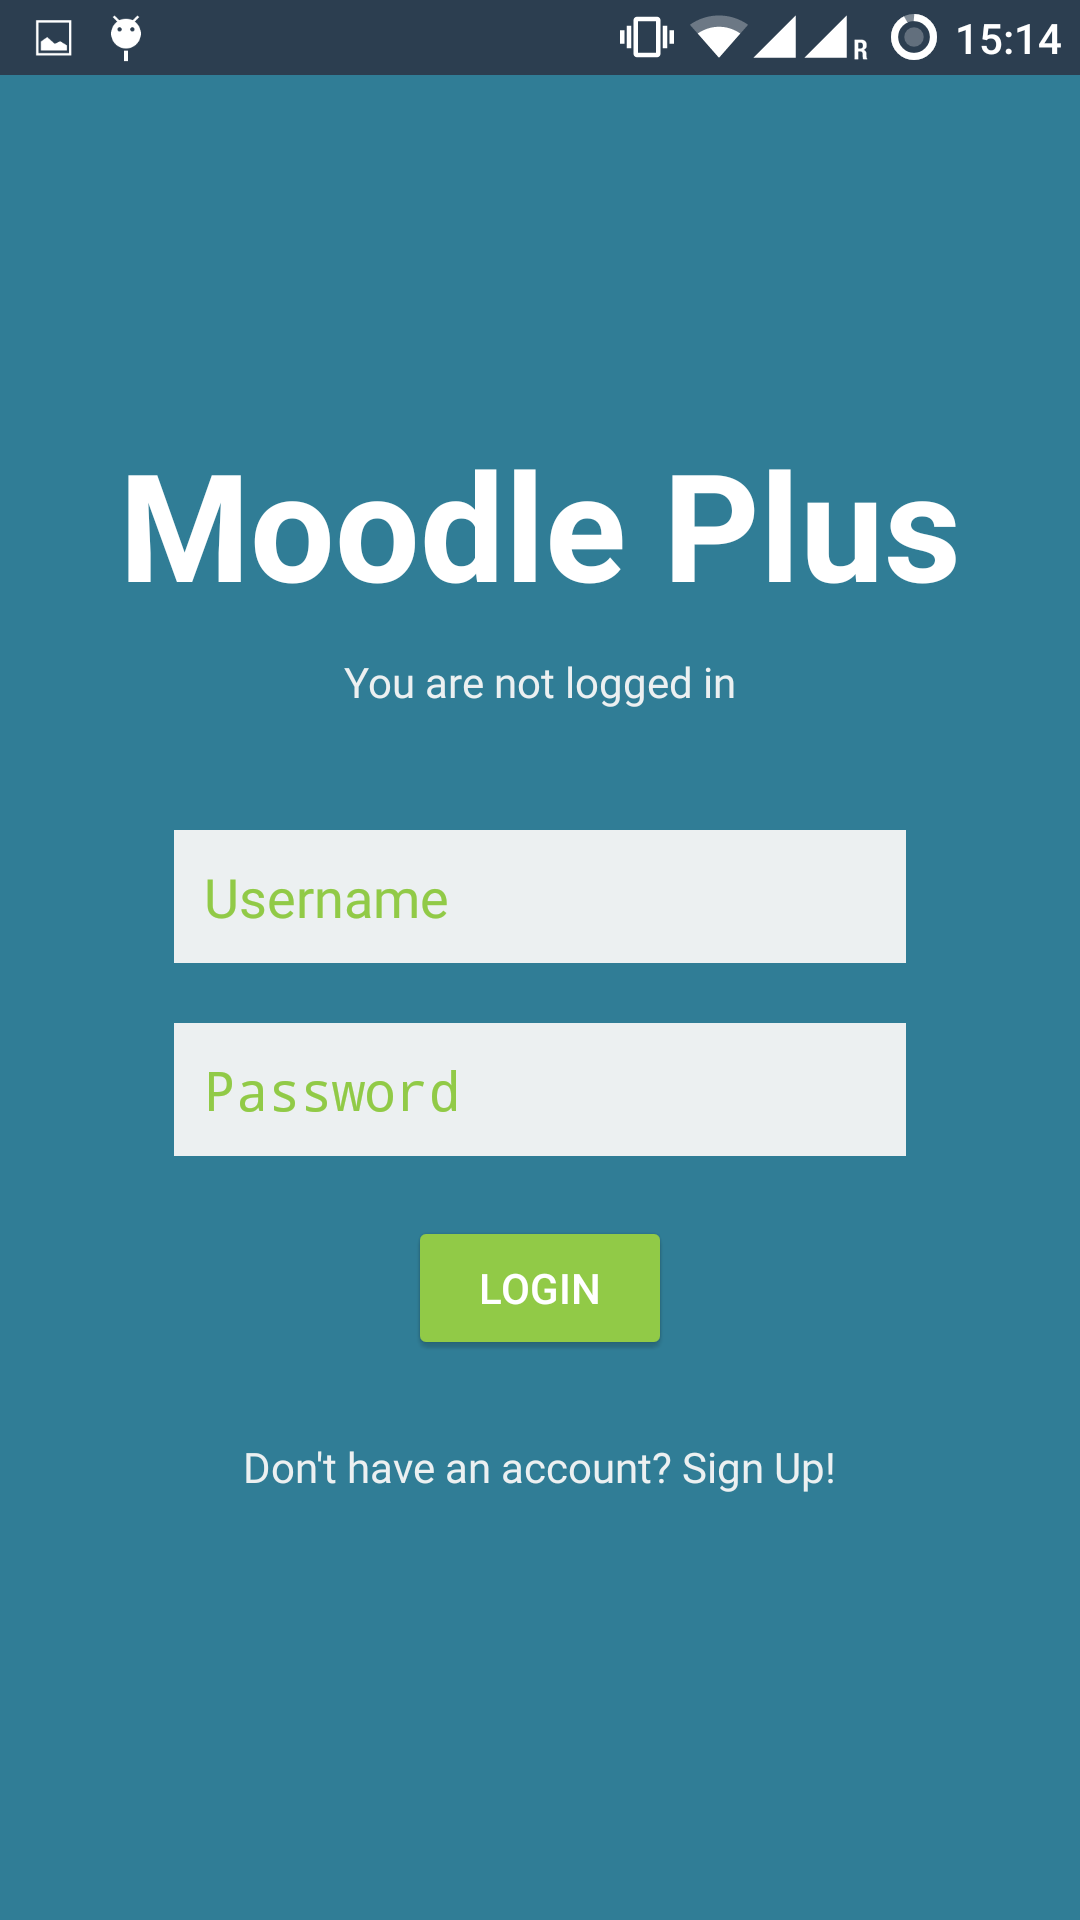
\includegraphics[scale=0.1]{login} 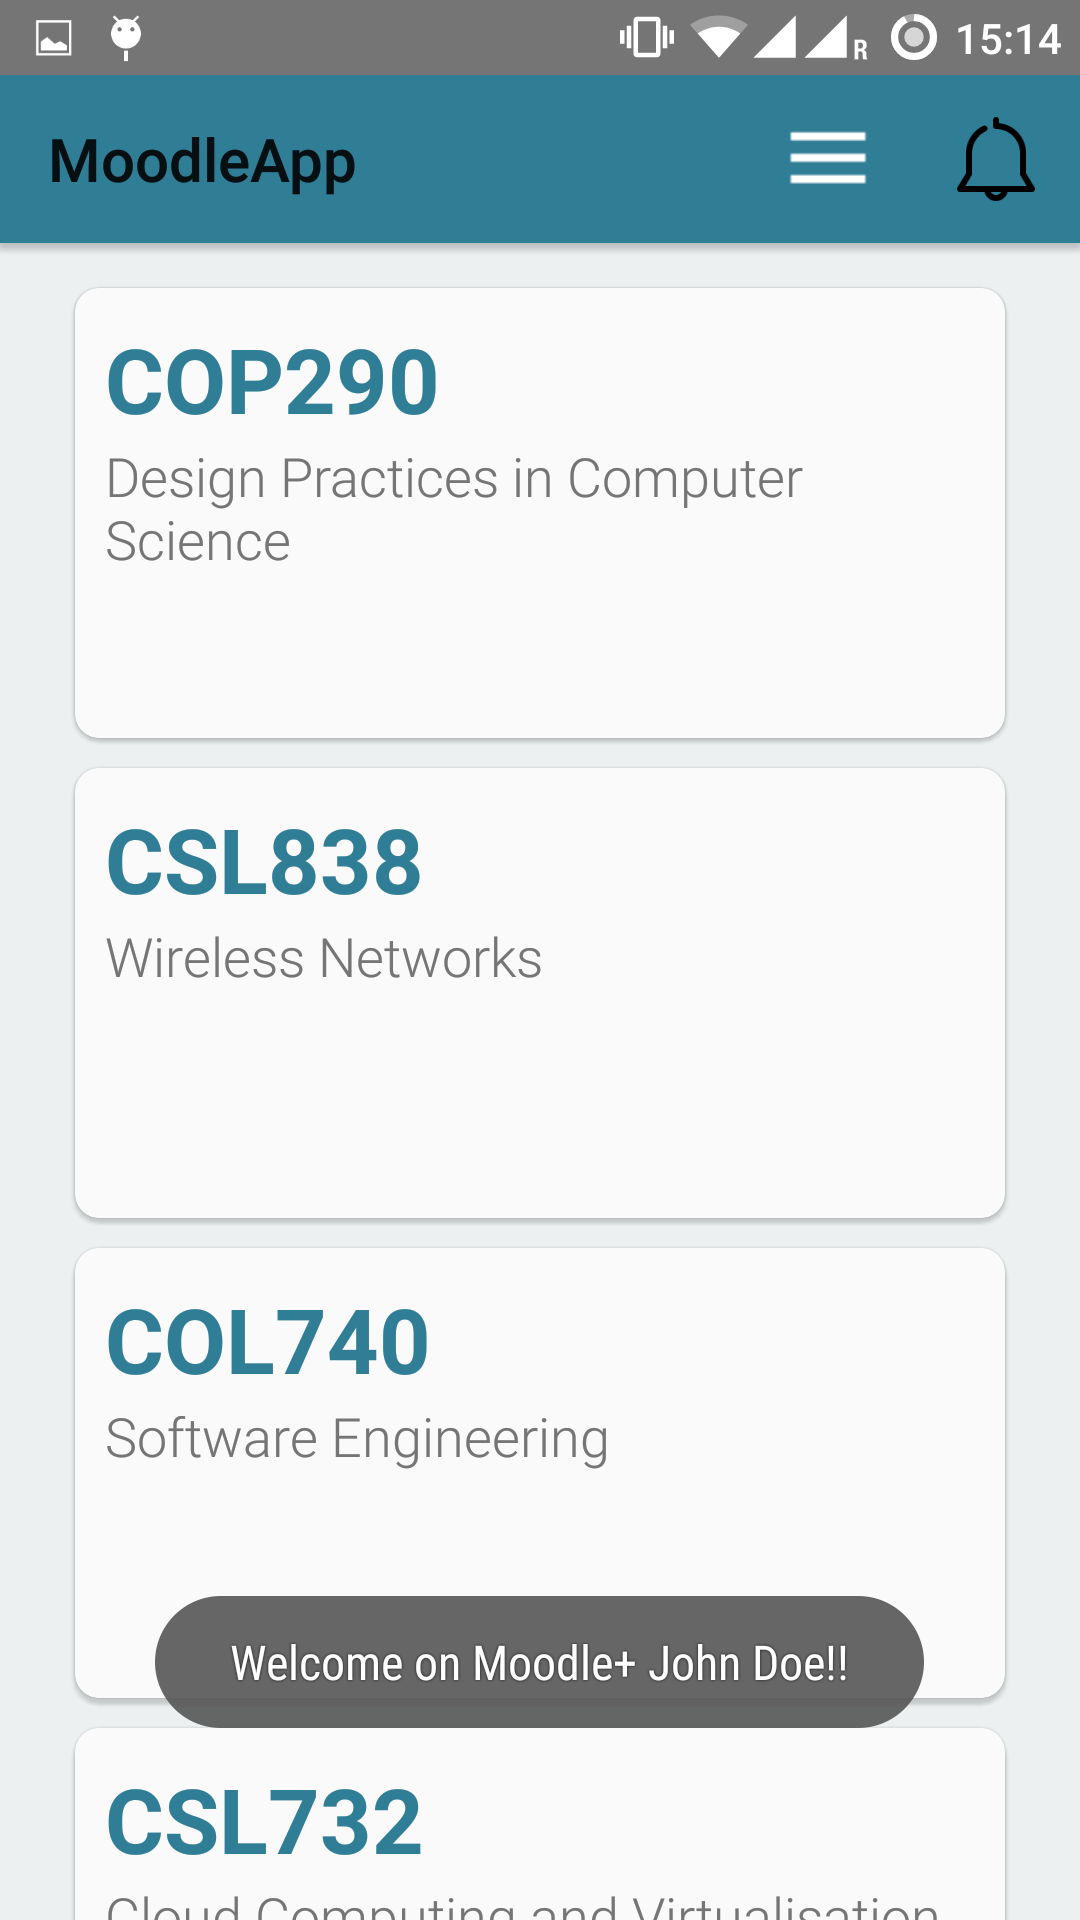
\includegraphics[scale=0.1]{mycourses} \\
On entering the right user name and password the user is logged in and taken to the my courses screen. This is a recycler-view with cards and each card displays the courses he/she is enrolled in(or in case of professors, has access to).
\item Course menu\\
On clicking on any of the courses, the user is taken to the menu of that particular course. From here the user can choose to see any of the items listed related to the course, for example, as shown he/she can see assignments, threads and resources related to that particular course\\

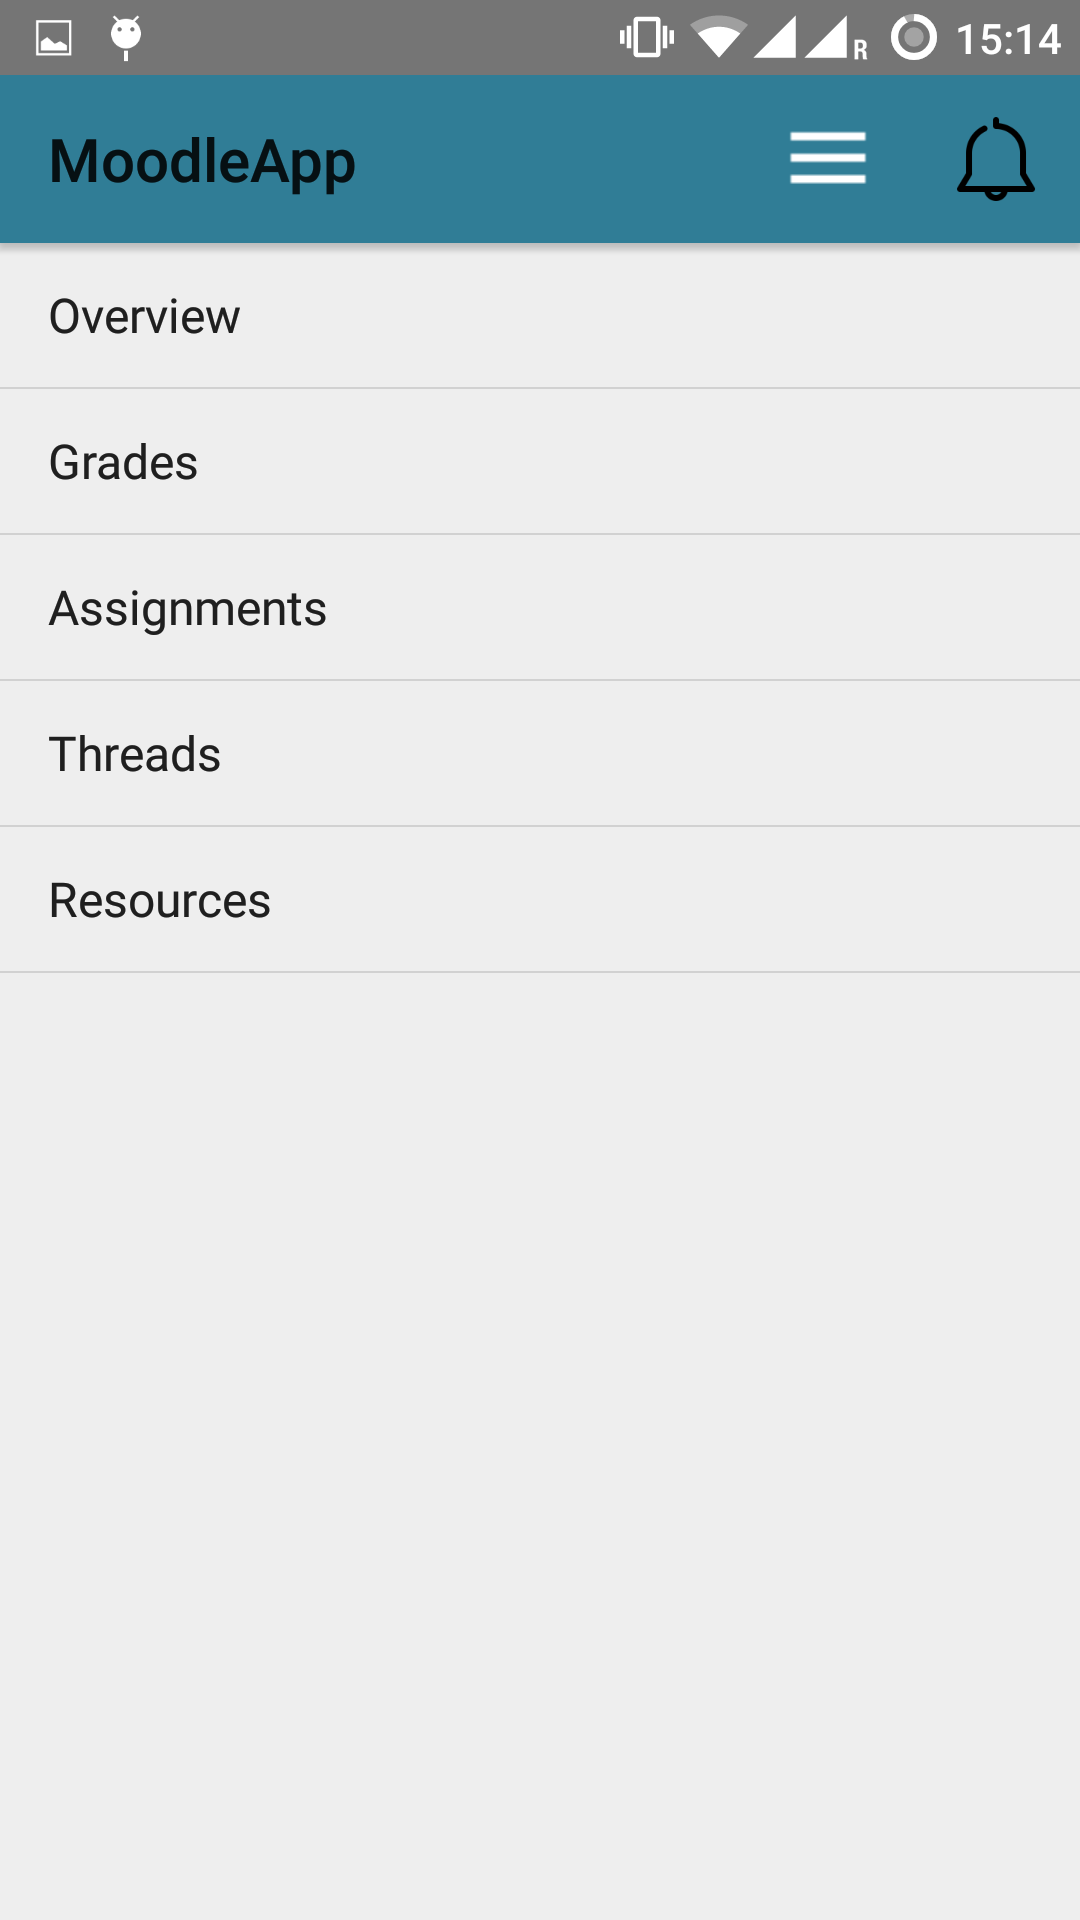
\includegraphics[scale=0.1]{coursemenu} \quad 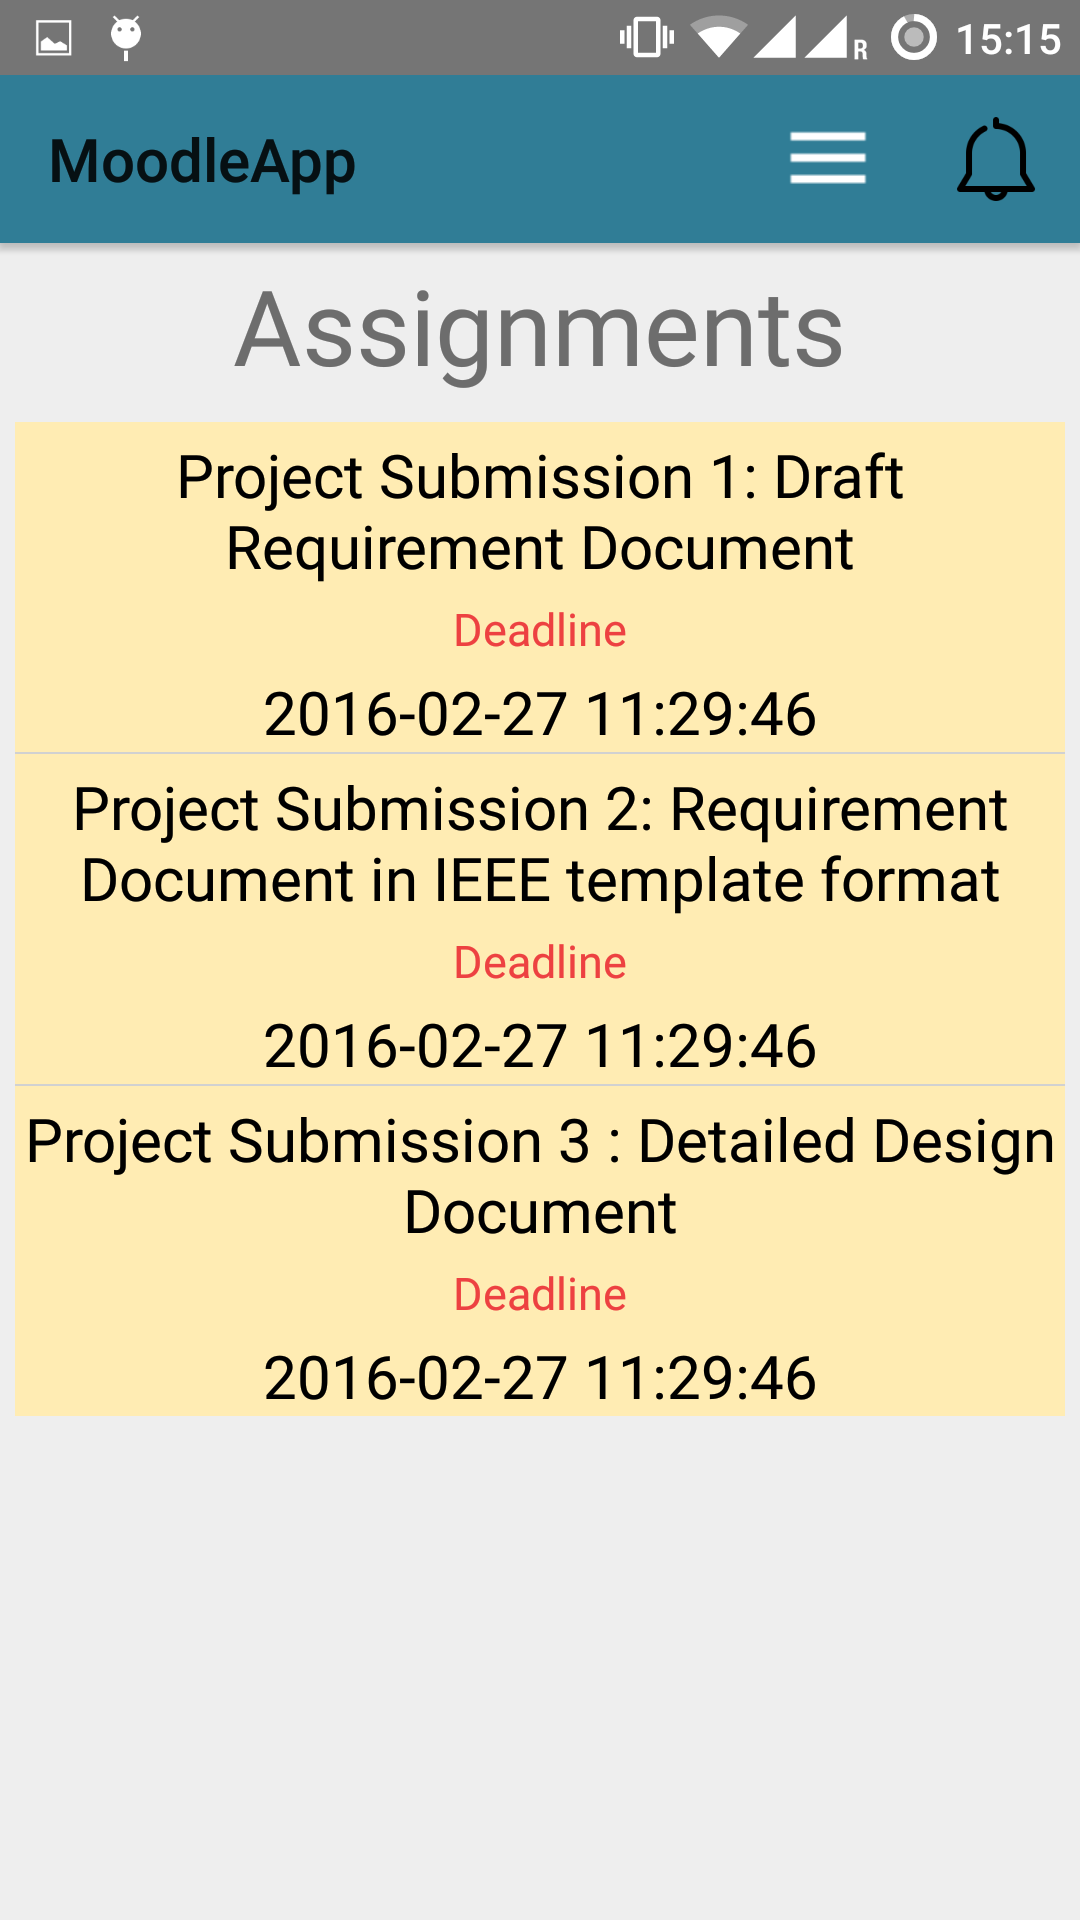
\includegraphics[scale = 0.1]{assignments} \quad 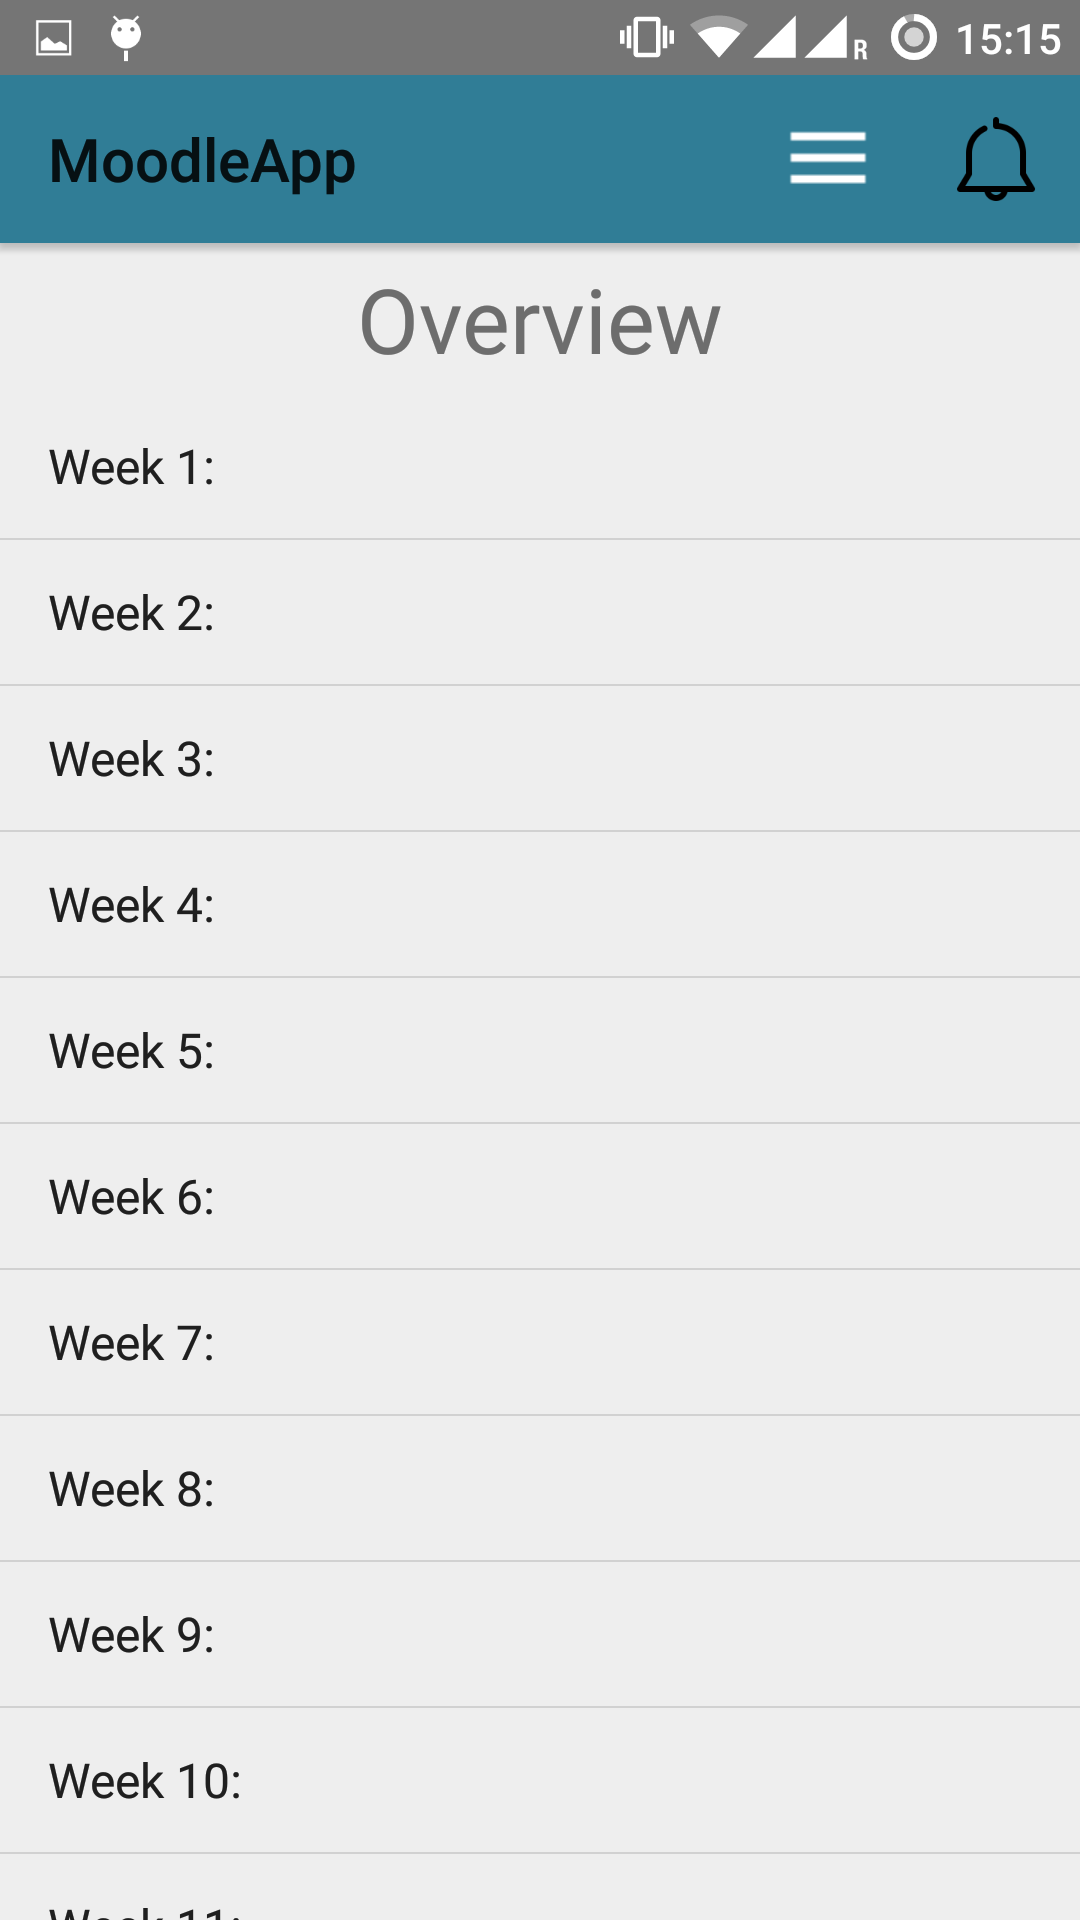
\includegraphics[scale=0.1]{overview}

\item Toolbar options\\
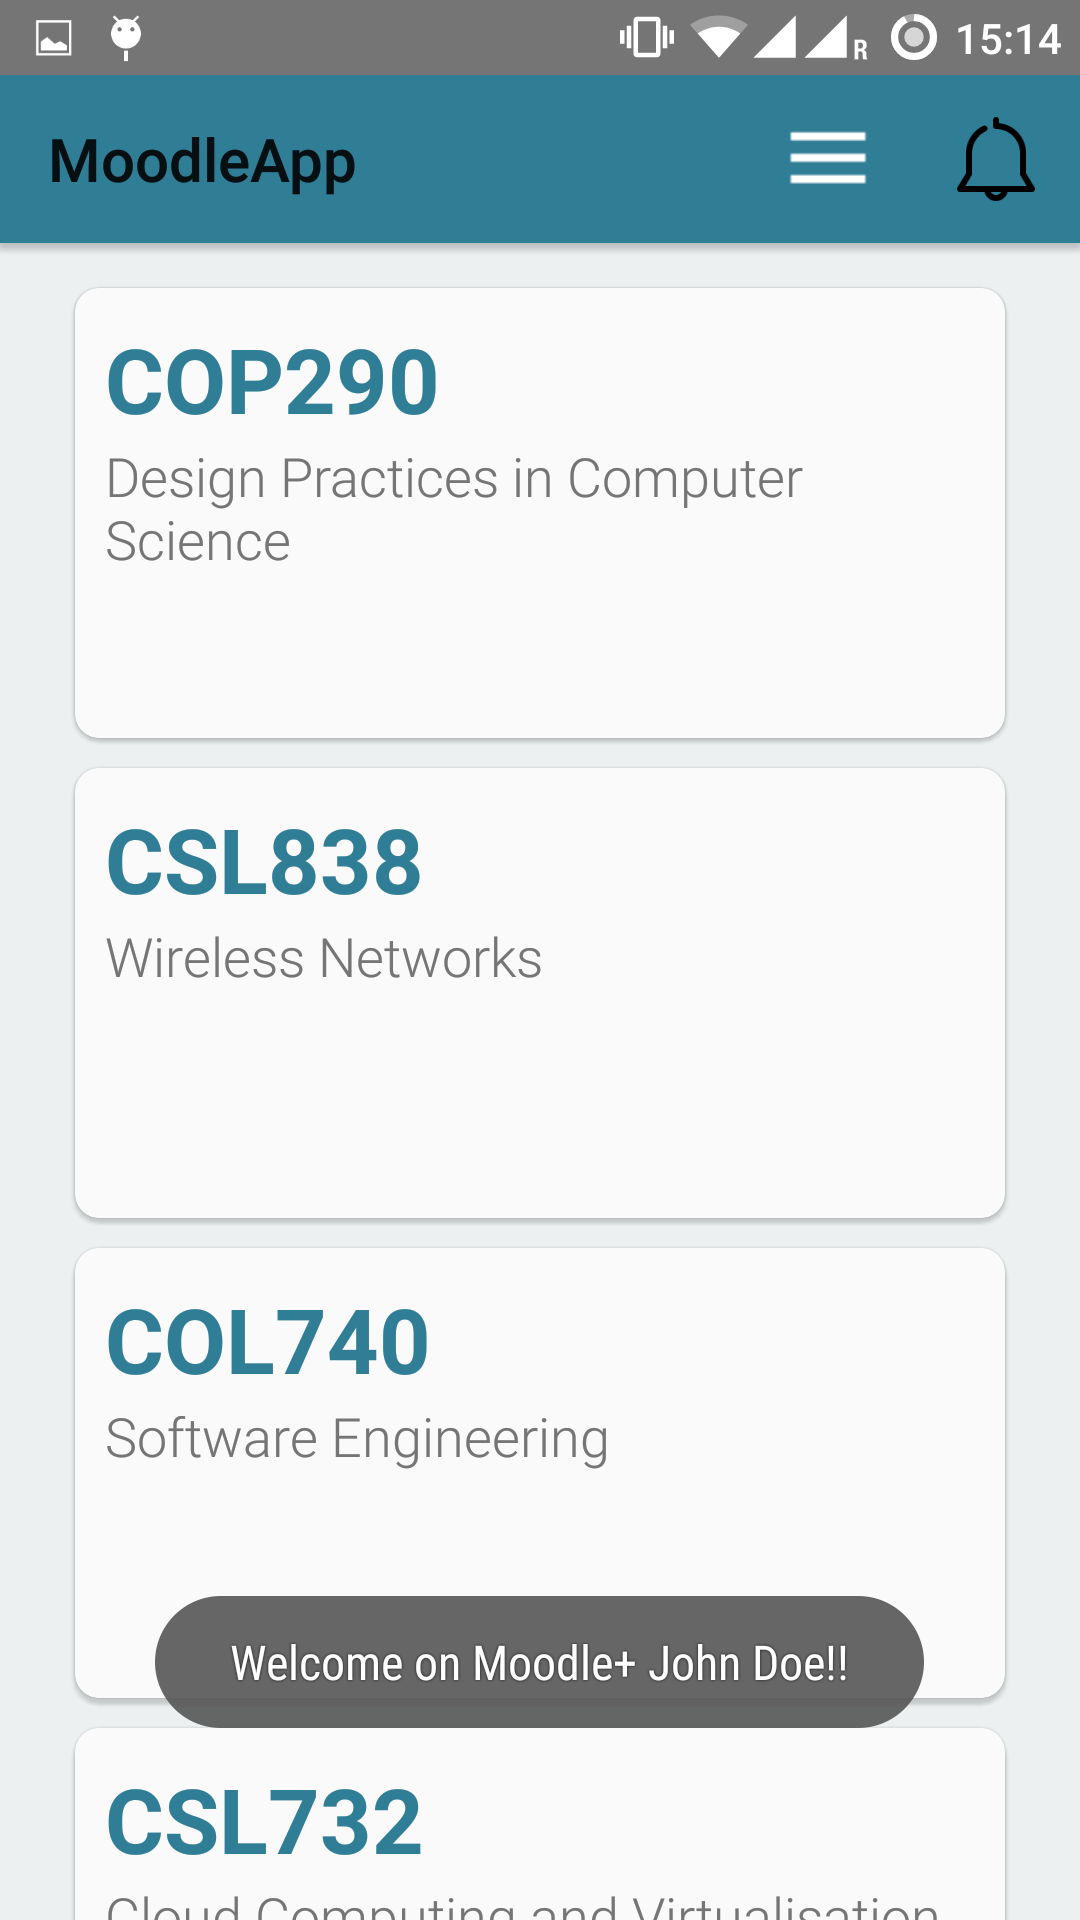
\includegraphics[scale=0.1]{mycourses} \quad \quad 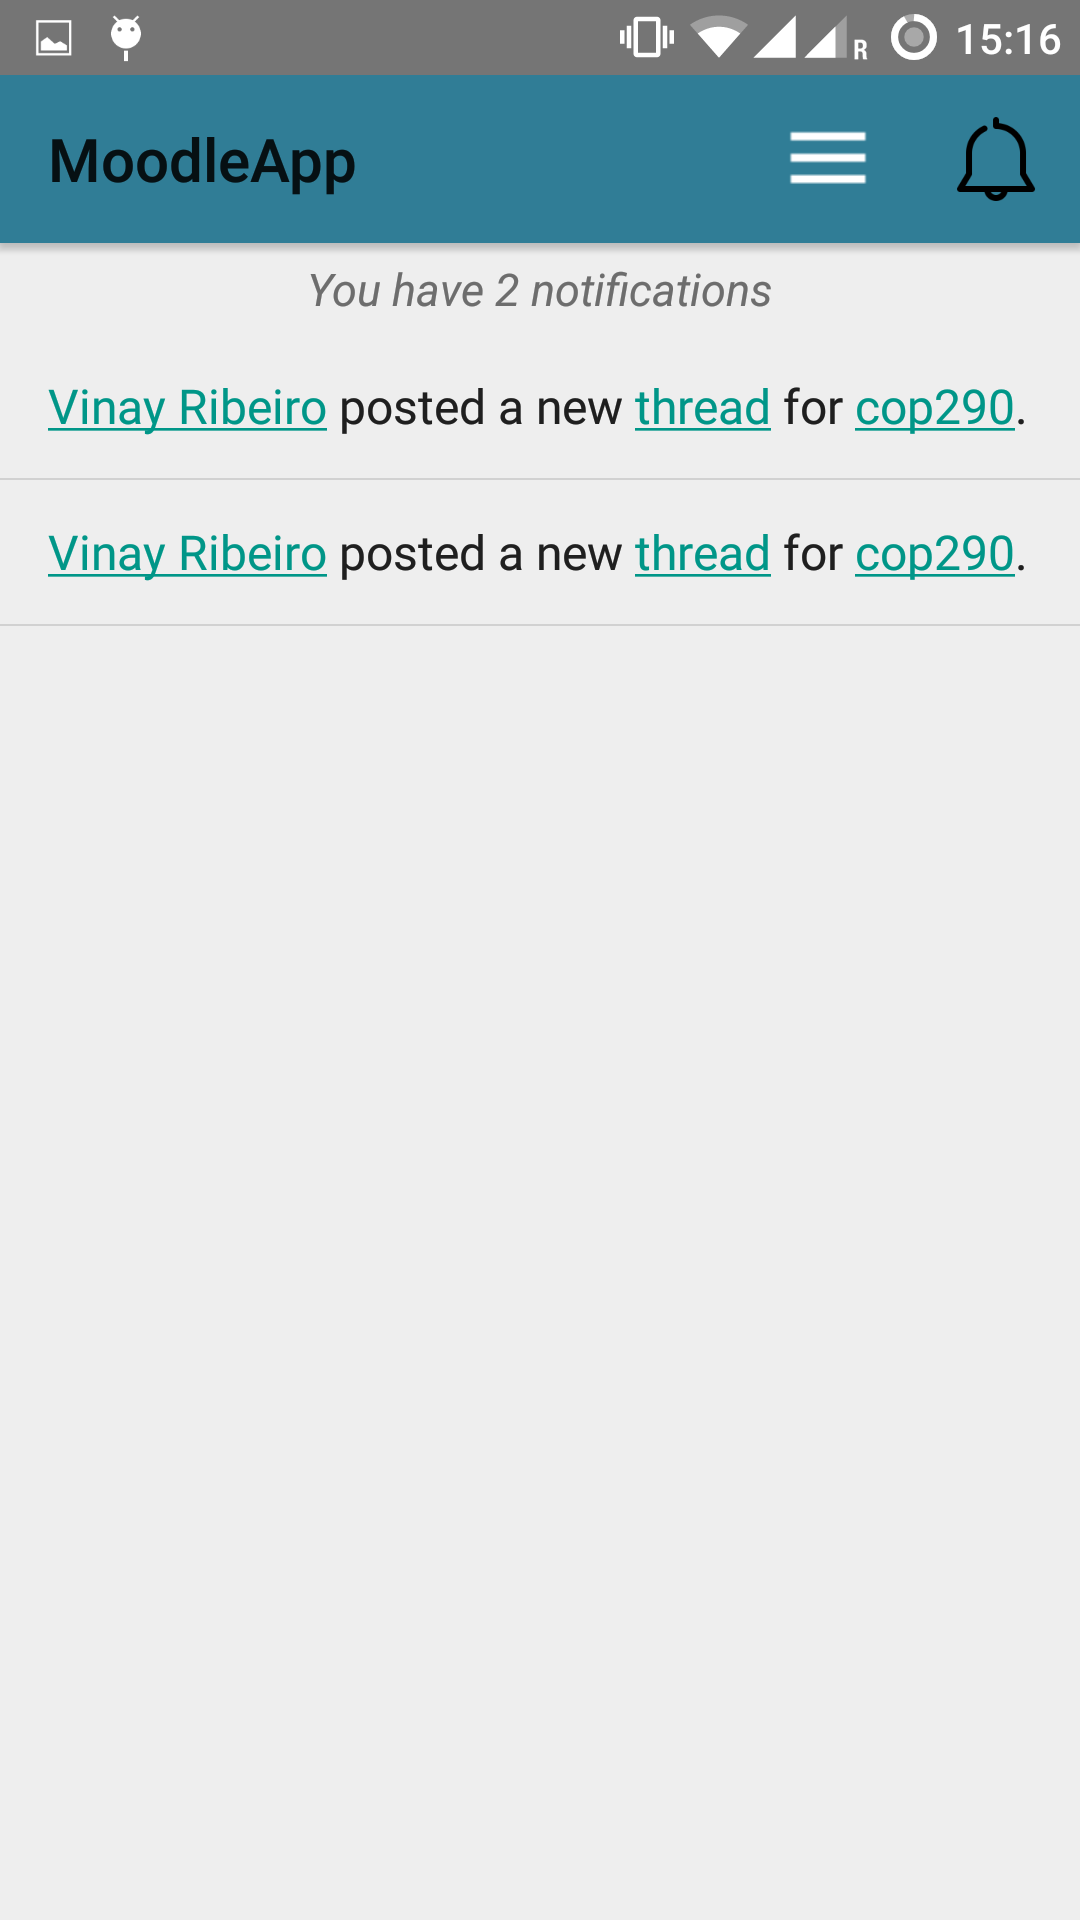
\includegraphics[scale=0.1]{notifications}\\
As can be seen from the screen attached, there is always a toolbar at the top which helps the user to open the drawer using the "hamburger" icon or open the notifications using the "bell" icon


\item Navigation Drawer \\
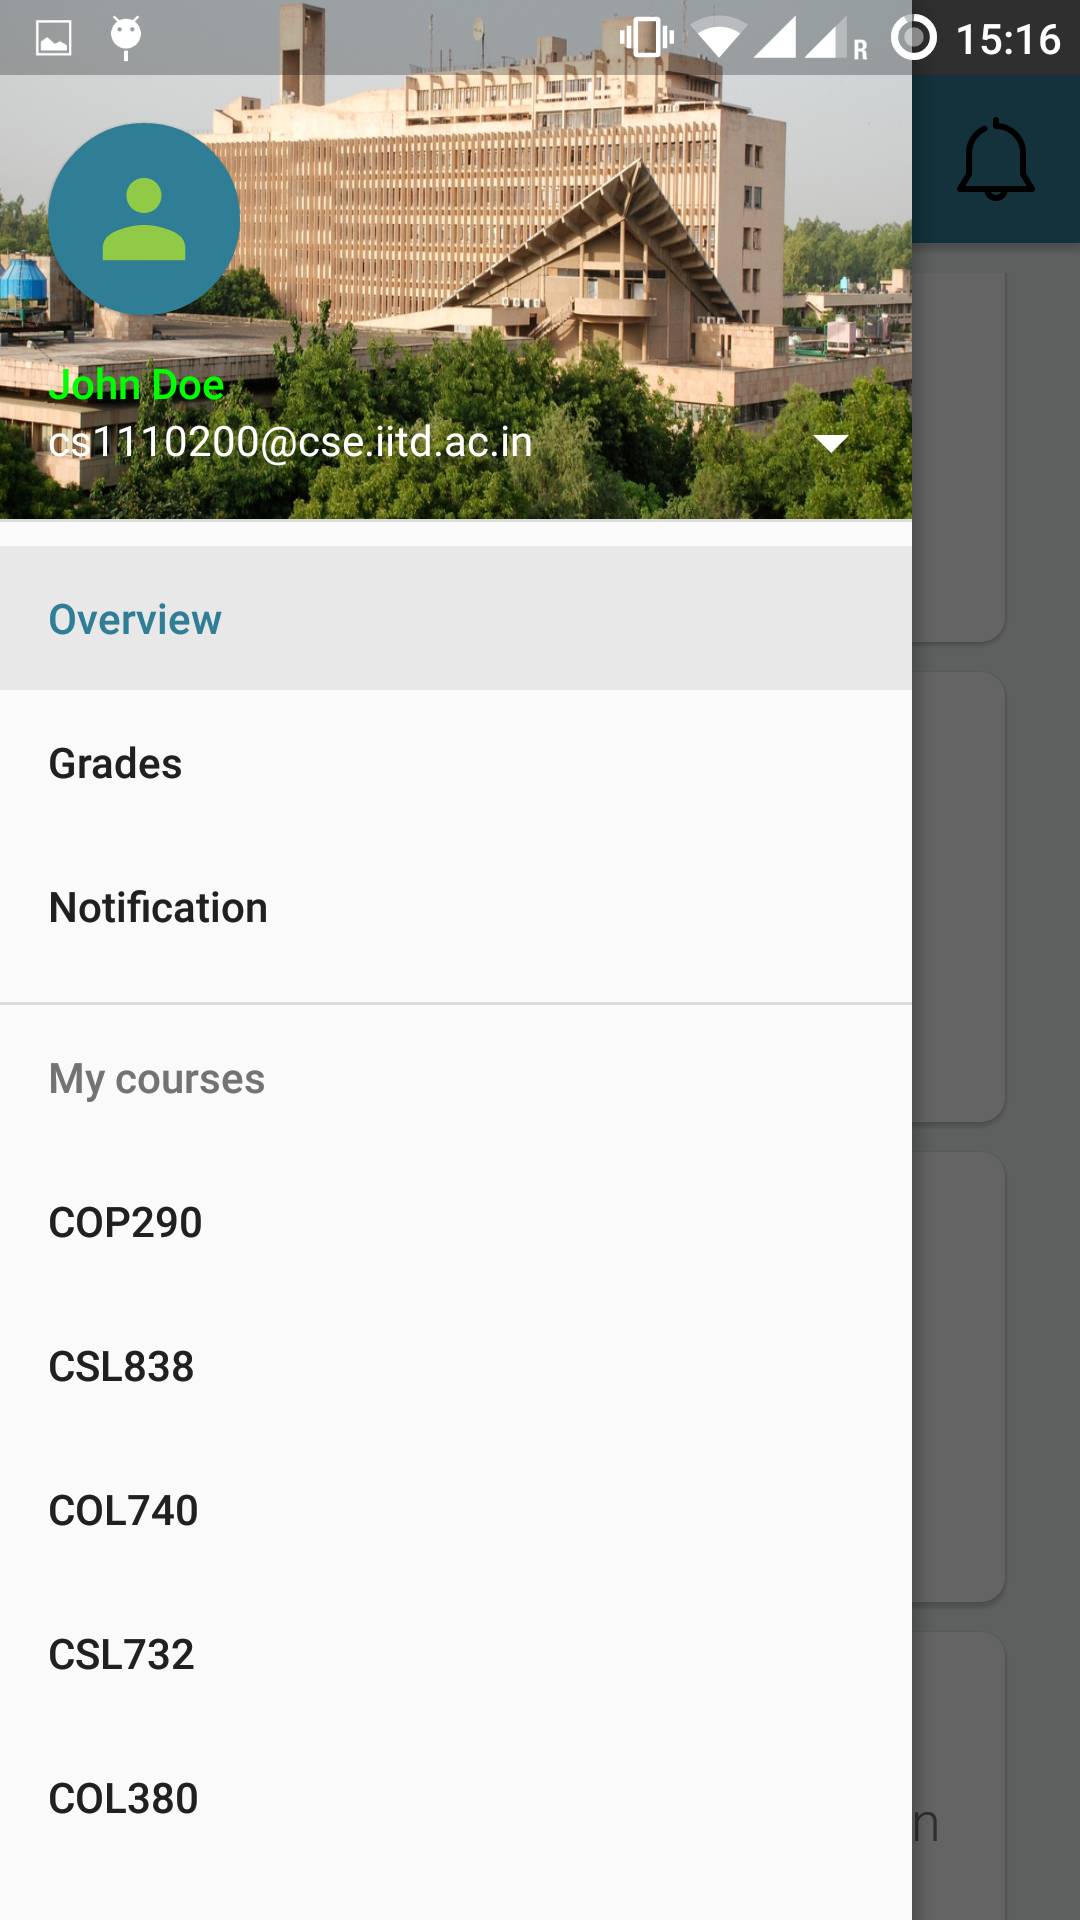
\includegraphics[scale = 0.1]{drawer} \quad 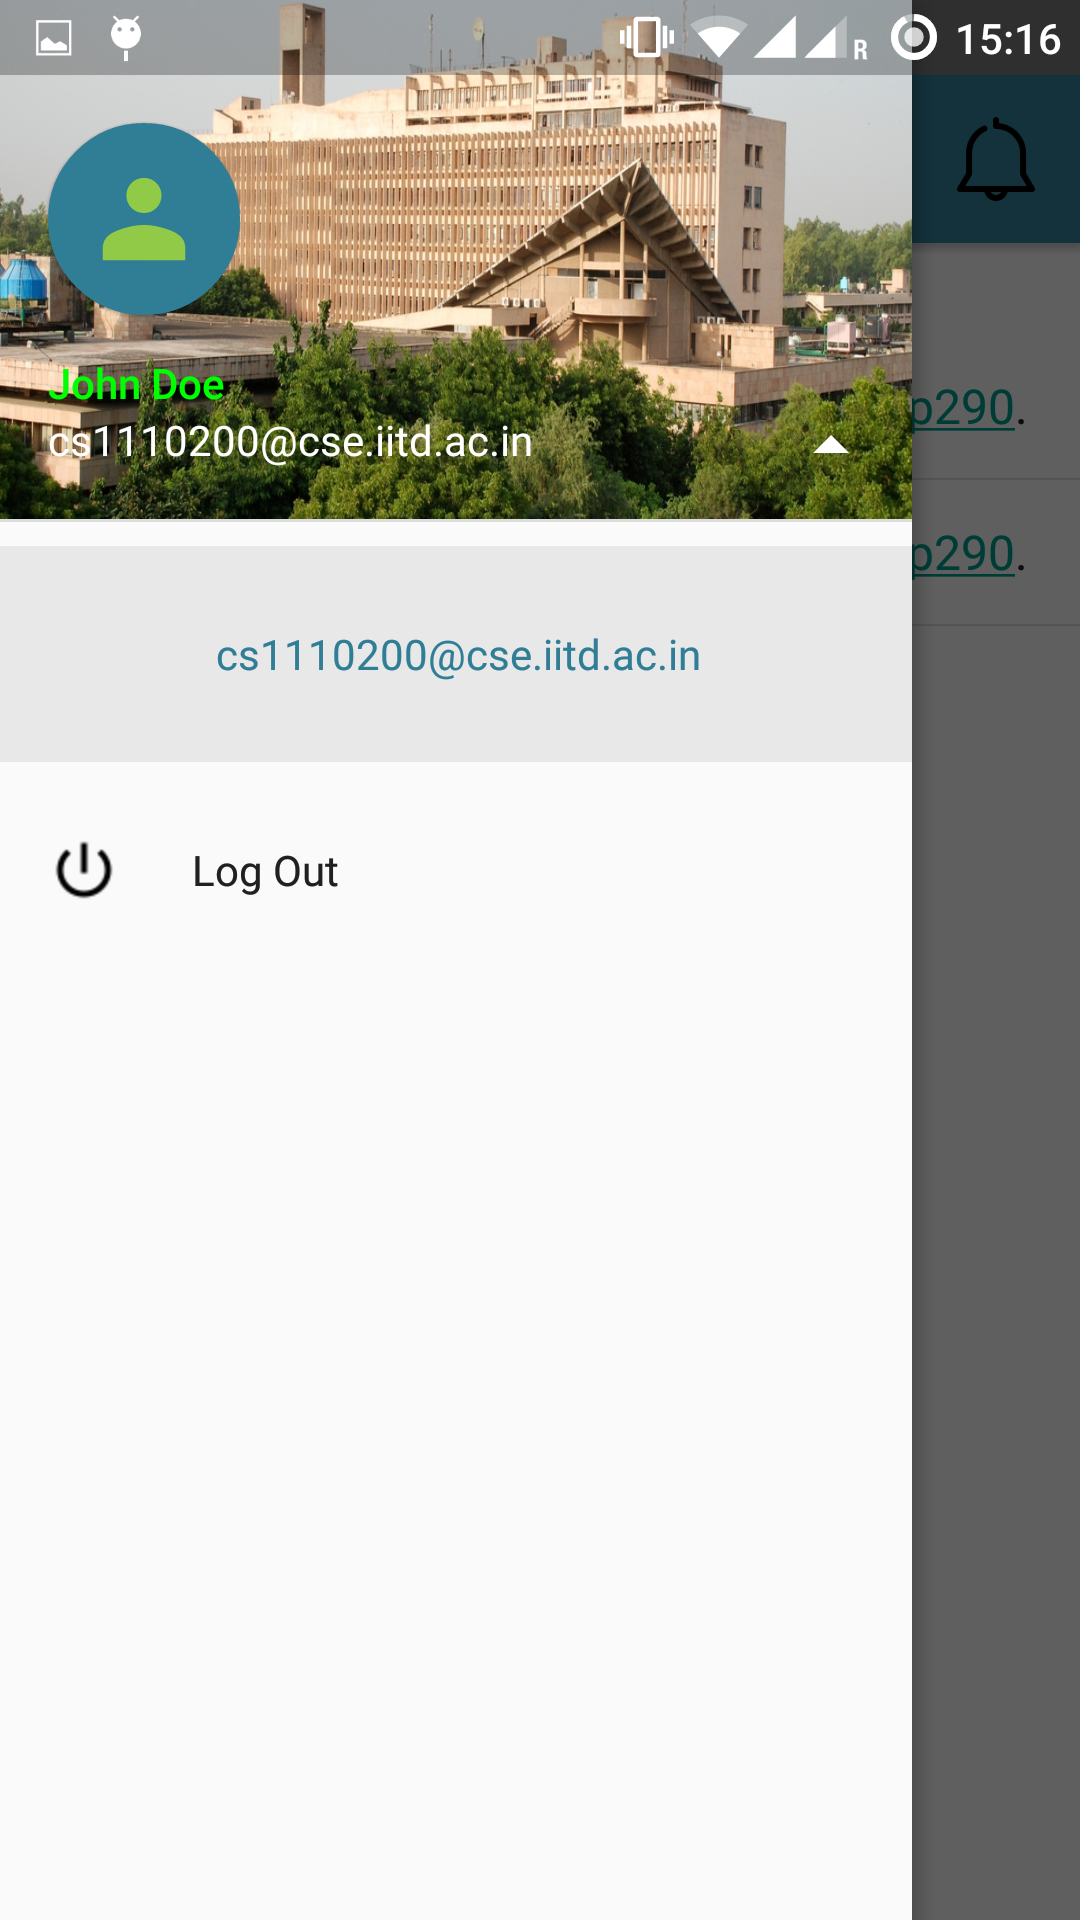
\includegraphics[scale=0.1]{logout} \\
For easy navigation, there is also a drawer in all screens of the app, so that user can switch to any of the screens when and as he/she wishes. Also, there is a logout button given n the user's profile button so that user can logout and login again\\
\end{itemize}


\section{Detail of Each activity or fragments}
\begin{itemize}
\item \textbf{MainActivity}\\
This is the main login screen that the user uses to enter his username and password. Also if the user doesn't have an account he is taken to the Signup activity.
when the user clicks on the submit button his details are sent in a string request,the cookies are stored and the response is sent to the next activity that is the \textbf{main2activity.java}\\
\item\textbf{Main2Activity}\\
This is the base activity for all the various fragments in the app and all the transcations are handled in this activity all buttons in this are linked to a request whose response is sent to the next fragment and the transaction is added to the backstack.This activity also holds the navigation drawer and the toolbar which all fragments share.
\item \textbf{MainActivityFragment} this fragmetn contains the recycler view which holds the cards of each course and onClick listener for each of the course, which sends him to the CourseFragment.
\item \textbf{CourseFragment} this contains the menu for each of the courses. As soon as the fragment is created the data sent by previous fragment is extracted ad then requests for each of the buttons here are created. When any of the listeners notice a click then the particular course information and the selected option specific data is combined into one url and the response of the stringrequest is sent to the next fragment on a successful request

\item \textbf{OverviewFragment, AssignmentFragment, GradesFragment, NotificationFragment} \\
All these fragments implement fragments which contain a list views and display the response from previous fragment after performing various formatting on them. So each of these have their own extensions of the arrayadapter to display the data received in the best possible way.
\item \textbf{ResourcesFragment} This fragment also essentially belongs to the same class of above fragments because this is also an endpoint in the application. Here the user can choose, by clicking the add file button any resource from their mobile directory.
\end{itemize}

\section{References and Resources used}
\begin{itemize}
\item We used the material design library by Google for various UI elements like the recycler view.
\item We also used MikePenz's material drawer library for the navigation drawer.
\item To read about how to implement various elements, we used websites like Vogella, Developer.android.com and extensively used StackOverFlow.
\end{itemize}
\end{document}
